\documentclass[a4paper,11pt,twocolumn]{article}
\usepackage[utf8]{inputenc}
%\usepackage[italian]{babel}

%\usepackage{lipsum}
\usepackage{float}
\usepackage{graphicx}
\usepackage[font=small,labelfont=bf]{caption}
\usepackage{multirow}
\usepackage{hyphenat}
\usepackage{sectsty}
%\usepackage{subfigure}
%\usepackage{color}
%\usepackage[dvipsnames]{xcolor}
%\sectionfont{\bfseries\Large\raggedright}
\usepackage{hyperref}
\allsectionsfont{\raggedright}
\graphicspath{ {images/} }

%\bibliographystyle{apalike}
\usepackage[dashed=false, maxnames=1, uniquelist=false, backend=bibtex,sorting=none,style=authoryear-icomp]{biblatex}
\renewbibmacro{in:}{}
\setlength{\bibhang}{0pt}
\renewcommand*{\bibfont}{\small}
\renewcommand*{\finentrypunct}{}
\addbibresource{bibliography.bib}

%\usepackage[T1]{fontenc}

\pagestyle{headings}


\title{Detection of a transiting Hot Jupiter around WASP-44}
\author{Adriana Barbieri \and Alessandro Bianchetti}

\begin{document}
\maketitle

\begin{abstract}

\emph{In the following report we work on WASP-44 b, an exoplanet orbiting 
arounf its G-type mother star, located in the constellation of Cetus. 
We first take a look at its atmospheric parameters and derive mass and 
radius (\cite{Morton}). Then, we correct for limb darkening effect in different ways 
(\cite{claret2011}, \cite{claret2017}, \cite{claret2018}). We also take 
some images taken by Copernico at the Asiago Observatory into consideration 
and, after proper correction, we use them to extract the light curve of 
the alleged planet.}

\end{abstract}

\section{Introduction}

Confirmed exoplanets are growing in number year by year, and transit method 
is nowadays a widely spread method. Most planets nowadays are discovered 
by tracing the lightcurve and searching for any sign of a weakening in the 
flux.
\begin{figure}[H]
    \centering  
    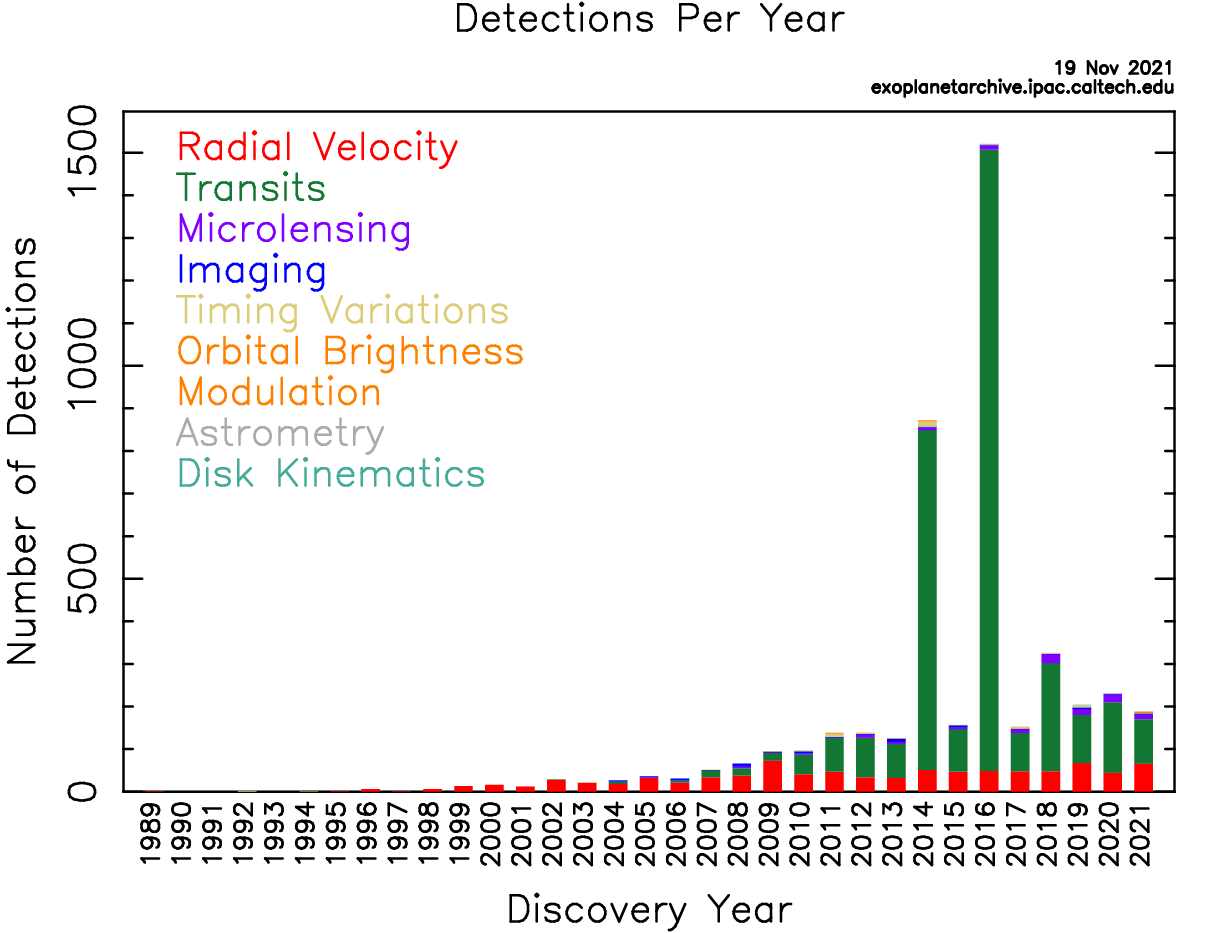
\includegraphics[scale=0.15, angle=0]{../pictures/exo_dischist.png}
    \caption*{\textit{ https://exoplanetarchive.ipac.caltech.edu/}}
\end{figure}
In this report we focus on WASP-44 b, a Jupyter-size planet orbiting around 
a G-type star, located in the constellation of Cetus.
Among the numerous available reports on the planet, we decided to make a 
conservative choice and avoid any result which is not inferred via 
spectroscopy. This leads us to rule out several papers about the object, and 
only work with the discovery paper (\cite{Anderson}). In this paper, estimates 
of the atmospheric parameters of WASP-44 are provided via an analysis of 
the width of spectral lines.

%\section{Instruments}




\section{Theoretical recap}

TODO
\begin{itemize}
    \item a brief overview of the transit method
    \item a comment on the bias of the transit method (big planets, close to the star)]

\end{itemize}


\section{Data analysis}

\subsection{Inferring mass and radius}

The $H_{\alpha}$ line was used to determine the effective temperature (Teff ),
while the $NaI$ D and $MgI$ b lines were used as surface gravity
($\log{g^*}$) diagnostics (\cite{Anderson}). The elemental abundances, including $[Fe/H]$ 
were determined from equivalent width measurements of several clean and 
unblended lines. This led to proper estimation of the atmospheric parameter 
triplet $T_{eff}$, $\log{g^*}$ and $[Fe/H]$. Quoted errors include statistical 
uncertainties only. In the same conservative spirit we 
previously showed, we add in quadrature a further term to the errors of 
all three parameters (\cite{Sousa}). We're in fact more interested in an 
accurate result rather than a precise one.
This leads to the following results 
\begin{center}
    \begin{tabular}{|c|c|c|}
    \hline
    $T_{eff}$ (K) & $\log{g^*}$ & $[Fe/H]$ \\
    $5400 \pm 162$ & $4.5 \pm 0.2$ & $0.06 \pm 0.11$ \\
    \hline
    \end{tabular}
    \end{center}


\subsection{Limb darkening correction}

Limb darkening is an important effect when observing a star, 
everything but negligible. In short, the edges of the luminosity profile 
of a star always look darker: this is because there is a physical, constant 
distance $L$ at which optical depth is equal to unity, further than which 
we cannot observe (photons do not reach us). This characteristic size, 
however, can go deep inside the hot layers of the star if we look straight 
to the center, being $L$ radial, while it can stop at colder, outer layers 
if we look at the edges of the star, since $L$ and our LOS are not radial 
anymore.
\begin{figure}[H]
    \centering  
    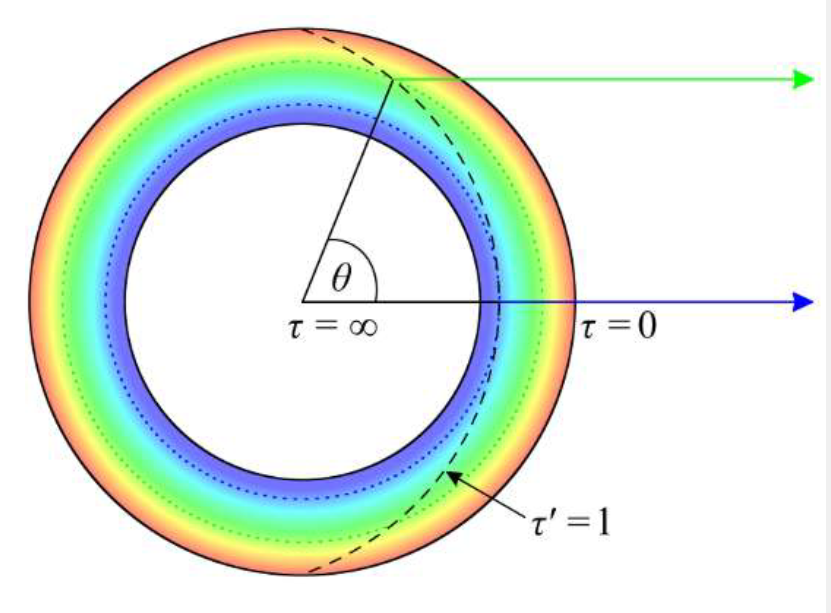
\includegraphics[scale=0.25, angle=0]{../pictures/limb_darkening.png}
    \caption{Limb darkening effect scheme. Credits to \textit{https://ediss.sub.uni-hamburg.de}}
\end{figure}
Correcting for this effect may be challenging. In fact we can measure it 
directly only for the Sun, while we need to model it somehow for any other 
star, meaning figure out a proper law for the intensity decrease $I(\mu)$, 
where $\mu = \sqrt{1-r^2}$. Many choices are plausible at this point: a 
uniform behaviour, a linear, a quadratic, a square-root or a 
logarithmic law are all valid guesses. Parametrizing such laws introduces 
the so-called \textit{LD-coefficients}, which will depend on the stellar 
parameters. Knowing the latter relationship (for instance calibrating it 
based on a large sample of stars) allows to obtain the coefficients directly 
from the atmopsheric parameters. 
The alternative way is fitting the light curve leaving the coefficients free.

The choice of the functional dependence on $\mu$ is a delicate one. Multiple 
approaches can be followed, basing on different papers. This analysis is 
tackled in \ref{sect:app_A}.


\subsection{Bias and flat field correction}
CCD (Charged Coupled Device) are the privileged detectors for photon counting, 
thanks to their great quantum efficiency. The images produced are \textit{raw}
and must be properly \textit{pre-reduced} before being analysed. Pre-reduction 
goes through different steps:
\begin{itemize}
    \item \textbf{bias} is the
    individual pixel-to-pixel offset level, and it's a zero-exposure instrumental 
    factor, thus it's always an added contribution to any signal. Therefore it must 
    be removed to isolate the photons of astrophysical origin. The root mean square 
    of the bias corresponds to the so-called \textit{readout noise}. We perform an 
    average out across all the pixels to get an estimate of the bias;
    \item a \textbf{flat field} is a calibration image obtained by illuminating
    homogeneously the pupil of the telescope, using twilight sky or appropriate, 
    back-lighted screens. This correction factor is to be applied on each pixel and 
    then also normalised, after the overall bias correction;
    \item \textbf{differential photometry} is a great way to keep track of any noise
    variation. The idea is to take a reference star close enoguh to the target: any 
    environmental or instrumental variation will affect both sources. Working with 
    flux ratios will make only astrophysical variations evident!
\end{itemize}
For pre-reductions steps, we use the code \textit{huggy}. We first perform bias
correction, than the flat field correction. The corrected images are ready for 
aperture synthesis.

\subsubsection{Bias correction}
We run \textit{huggy-bias.e} inputting the raw images. Many bias images are produced,
displaying the zero offset of the pixel board. \textit{Master bias} is the average 
of all these files. Plotting the intensities of offset level of the pixels yields 
a concrete view of the correction.
\begin{figure}[H]
    \centering  
    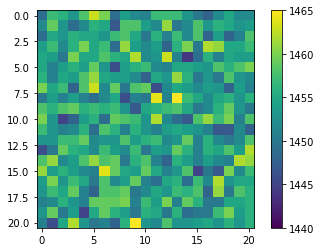
\includegraphics[scale=0.32, angle=0]{../pictures/pre-reduction/bias.png}
    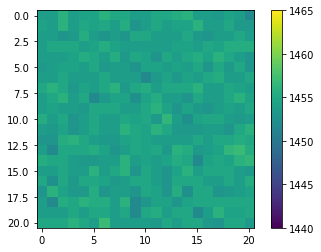
\includegraphics[scale=0.32, angle=0]{../pictures/pre-reduction/master_bias.png}
    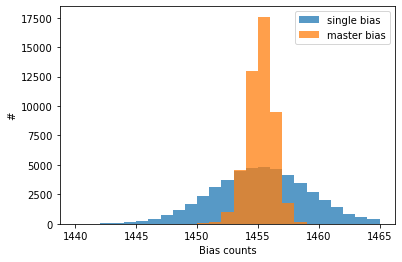
\includegraphics[scale=0.35, angle=0]{../pictures/pre-reduction/bias_comp.png}
    \caption{Comparison between random bias frame and master bias}
\end{figure}
Note that the master bias frame distribution is peaked and much closer to a 
unique constant value, as all pixels behaved in the same way, like in an 
ideal situation. We can see this even numerically, by looking at the 
dispersions of the above distributions: $\sigma_{rb} = 3.82$ and 
$\sigma_{mb} = 0.89$.


\subsection{Extracting the light curve}


\section{Conclusions}




\section{Appendix A: limb darkening analysis}
\label{sect:app_A}

\subsection{Claret 2017}
We can represent data tables in \cite{claret2017} as 2D histograms, 
after proper unfolding of the data tables attached to the paper. To do that, 
we first fix metallicity, then gravity and see how the corresponding LD 
coefficients $c_1$ and $c_2$ depend on all three atmospheric parameters. 
\begin{figure}[H]
    \centering  
    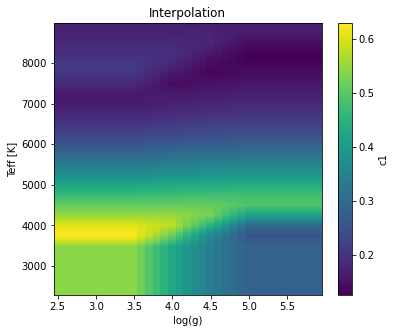
\includegraphics[scale=0.25, angle=0]{../pictures/Claret2017/2017_c1_fixedmet}
    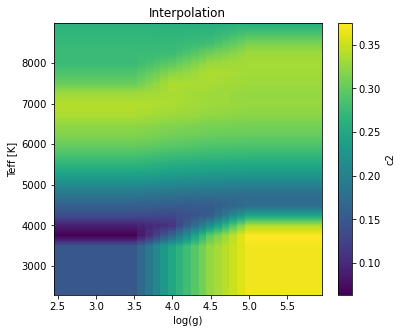
\includegraphics[scale=0.25, angle=0]{../pictures/Claret2017/2017_c2_fixedmet}

    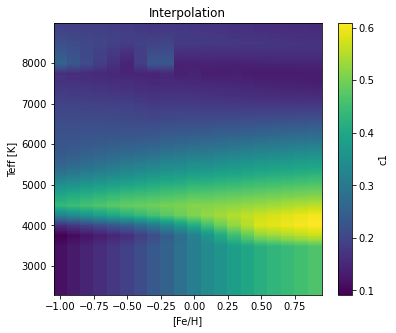
\includegraphics[scale=0.25, angle=0]{../pictures/Claret2017/2017_c1_fixedg}
    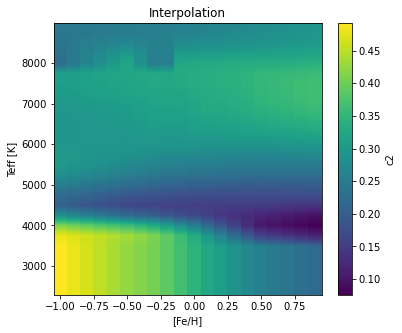
\includegraphics[scale=0.25, angle=0]{../pictures/Claret2017/2017_c2_fixedg}
    \caption{LD coefficient with fixed metallicty, fixed gravity}
\end{figure}
Furthermore, it's very interesting to check the strength of the dependance 
on each atmospheric parameters. Turns out LD coefficients are essentially a 
function of temperature, and minor dependences on gravity and metallicity 
can be barely appreciated.
\begin{figure}[H]
    \centering  
    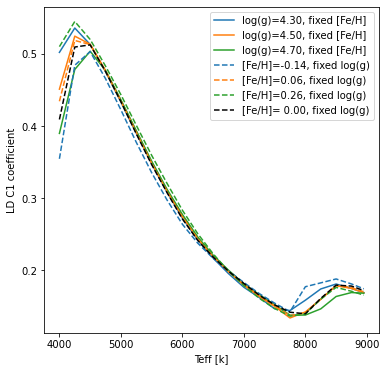
\includegraphics[scale=0.25, angle=0]{../pictures/Claret2017/2017_c1}
    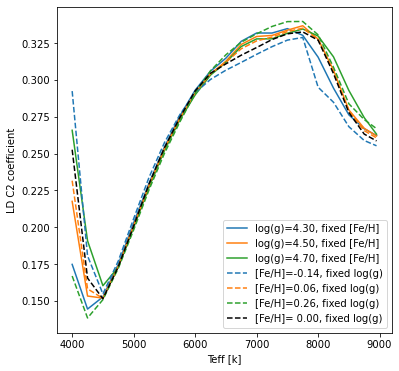
\includegraphics[scale=0.25, angle=0]{../pictures/Claret2017/2017_c2}
    \caption{LD coefficient as a function of atmospheric parameters}
\end{figure}
A relevant dependance on gravity and metallicity can only be noticed at 
high temperatures, where we should carefully select the proper curve. But 
in the range we're interested in ($\approx 5400 K$) the curve is 
degenerate and the choice of these parameters is secondary.

We perform a Montecarlo simulation, generating 1000 random atmospheric 
parameters around the actual ones. Even in this case we see that the 
distribution of the fixed-metallicity estimates is almost overlapping 
with the fixed-gravity one, thus confirming $c_1$ and $c_2$ not very 
sensitive on metallicity and gravity.
\begin{figure}[H]
    \centering  
    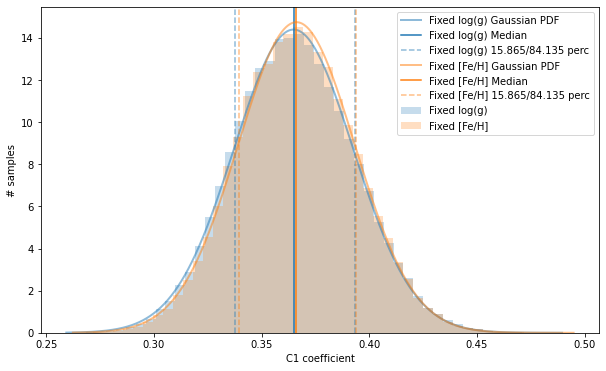
\includegraphics[scale=0.35, angle=0]{../pictures/Claret2017/2017_c1_comp}
    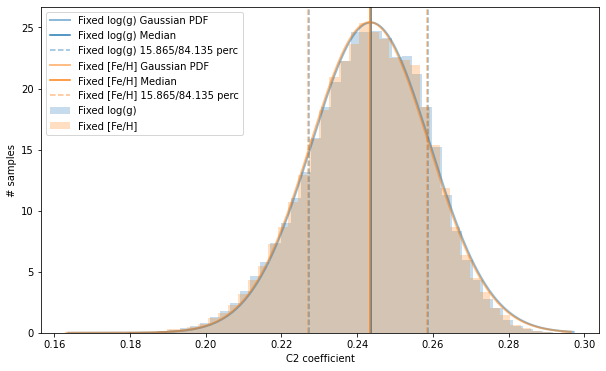
\includegraphics[scale=0.35, angle=0]{../pictures/Claret2017/2017_c2_comp}
    \caption{Montecarlo simulation for $c_1$ and $c_2$, for fixed metallicity 
    and for fixed gravity}
\end{figure}
The two estimates are well compatible, thus authorizing a weighted average: 
$c_1 = 0.366 \pm 0.019$ and $c_2 = 0.243 \pm 0.011$.

Another way to deal with the same table is by selecting from the set the two 
closest stars to ours, instead of just one. The rest of the procedure is 
the same as just explained, leading to other estimate of the LD coefficients.

\subsection{Claret 2018}
Only the zero metallicity case in now considered.


\printbibliography

\end{document}